\section{Graftyper}
Grafer kan opdeles i forskellige typer. Herunder simple grafer, multigrafer og pseudografer. Vi kigger først på en simpel graf.

\begin{defn}[Simpel graf] \label{defn:simpel}
En \emph{simpel graf}, $G=(V,E)$, består af $V$, en mængde knuder, hvor $V \neq \emptyset$, og en mængde kanter, $E \subseteq \{\{u,v\}|u,v \in V, u \neq v\}$, som opfylder $\nexists \ e_i, e_j \in E : e_i = e_j$.
\end{defn}

Det ses i Definition \autoref{defn:simpel}, at en kant i en simpel graf skal være incident med to knuder, der kan altså ikke optræde løkker. Foruden dette ser vi også, at der kun kan forekomme én kant mellem to knuder.

\begin{figure}[H]
\centering
	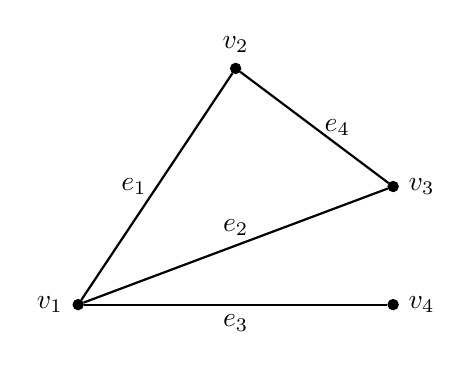
\begin{tikzpicture}

      \tikzset{enclosed/.style={draw, circle, inner sep=0pt, minimum size=.13cm, fill=black}}
%% Vertices
      	\node[enclosed, label={left: $v_1$}] (v1) at (0,0) {};
      	\node[enclosed, label={above: $v_2$}] (v2) at (2,3) {};
    	\node[enclosed, label={right: $v_3$}] (v3) at (4,1.5) {};
  	    \node[enclosed, label={right: $v_4$}] (v4) at (4,0) {};
%Edges
		\path[thick] (v1) edge node[midway, left] {$e_1$} (v2);
		\path[thick] (v1) edge node[midway, above] {$e_2$} (v3);
		\path[thick] (v1) edge node[midway, below] {$e_3$} (v4);
		\path[thick] (v2) edge node[midway, right] {$e_4$} (v3);

	\end{tikzpicture}
	\caption{Simpel graf.}
	\label{fig.simpel}
\end{figure}



I kontrast til den simple graf finder vi multigrafen, der skal indeholde flere kanter, som er incidente med samme knudepar. Hvis to kanter er incidente med samme knudepar, kaldes de \emph{parallelle}.

\begin{defn}[Multigraf] \label{defn:multi}
En \emph{multigraf}, $ G = (V,E)$, består af $V$, en mængde knuder, hvor $V \neq \emptyset$, og en mængde kanter,
$E \subseteq \{\{u,v\}|u,v \in V, u \neq v\}$, som opfylder $\exists \ e_i, e_j \in E : e_i = e_j$.
\end{defn}

\begin{figure}[H]
\centering
	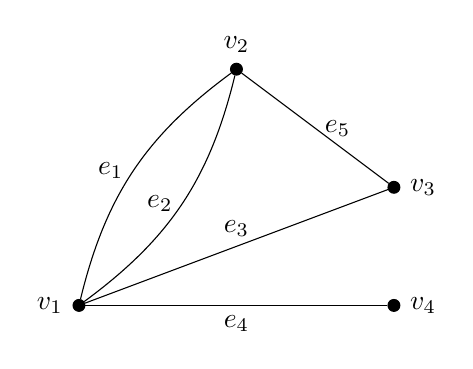
\begin{tikzpicture}

      \tikzset{enclosed/.style={draw, circle, inner sep=0pt, minimum size=.15cm, fill=black}}
%% Vertices
      	\node[enclosed, label={left: $v_1$}] (v1) at (0,0) {};
      	\node[enclosed, label={above: $v_2$}] (v2) at (2,3) {};
    	\node[enclosed, label={right: $v_3$}] (v3) at (4,1.5) {};
  	    \node[enclosed, label={right: $v_4$}] (v4) at (4,0) {};
%Edges
		\path (v1) edge [bend right=20] node[midway, left] {$e_2$} (v2);
		\path (v2) edge [bend right=20] node[midway, left] {$e_1$} (v1);
		\path (v1) edge node[midway, above] {$e_3$} (v3);
		\path (v1) edge node[midway, below] {$e_4$} (v4);
		\path (v2) edge node[midway, right] {$e_5$} (v3);

	\end{tikzpicture}
	\caption{En multigraf.}
	\label{fig.multi}
\end{figure}


I forlængelse heraf har vi pseudografen, som ingen krav har om mængden af kanter mellem to knudepar, derimod skal der eksistere mindst én løkke. 

\begin{defn}[Pseudograf] \label{defn:pseudo}
En \emph{pseudograf}, $ G = (V,E)$, består af $V$, en mængde knuder, hvor $V \neq \emptyset$, og en mængde kanter, $E \subseteq \{\{u,v\}|u,v \in V\}$, hvor $\exists \ e_i \in E$,S som opfylder $e_i = \{v,v\}$.
\end{defn}

Vi ser i eksemplet herunder, at der er to parallelle kanter mellem $v_{1}$ og $v_{2}$ og en løkke ved $v_{4}$.

\begin{figure}[H]
\centering
	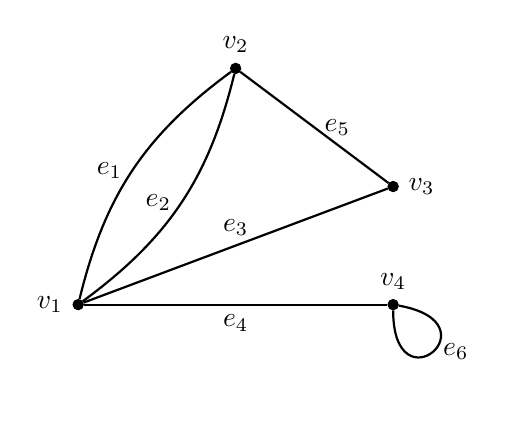
\begin{tikzpicture}[every loop/.style={}]
      \tikzset{enclosed/.style={draw, circle, inner sep=0pt, minimum size=.13cm, fill=black}}
%% Vertices
      	\node[enclosed, label={left: $v_1$}] (v1) at (0,0) {};
      	\node[enclosed, label={above: $v_2$}] (v2) at (2,3) {};
    	\node[enclosed, label={right: $v_3$}] (v3) at (4,1.5) {};
  	    \node[enclosed, label={above: $v_4$}] (v4) at (4,0) {};
%Edges
		\path[thick] (v1) edge [bend right=20] node[midway, left] {$e_2$} (v2);
		\path[thick] (v2) edge [bend right=20] node[midway, left] {$e_1$} (v1);
		\path[thick] (v1) edge node[midway, above] {$e_3$} (v3);
		\path[thick] (v1) edge node[midway, below] {$e_4$} (v4);
		\path[thick] (v2) edge node[midway, right] {$e_5$} (v3);
		\path[thick] (v4) edge [out=270,in=350,looseness=35] node[right] {$e_6$} (v4);
	\end{tikzpicture}
	\caption{Pseudograf med en løkke.}
	\label{fig.pseudo}
\end{figure}



\subsection{Orienterede grafer og ikke-orienterede grafer}
En anden typisk grafopdeling er opdelingen i \emph{orienterede grafer} og \emph{ikke-orienterede} grafer. De grafer, vi har kigget på indtil videre, er ikke-orienterede grafer. For en orienteret graf gælder det, at grafens kanter er retningsbestemte. Dette er ofte illustreret med pile. Den har dermed en startknude og en endeknude. Disse grafer er defineret ved:

\begin{defn} [Orienteret graf] 
En orienteret graf, $G=(V,E)$, består af $V$, en mængde knuder, hvor $V \neq \emptyset$, og en mængde orienterede kanter, $E$. Hver orienterede kant er incident med et ordnet knudepar, $(u,v)$, hvor kanten går fra startknuden, $u$, til endeknuden, $v$. 
\end{defn}

\begin{figure}[H]
\centering
	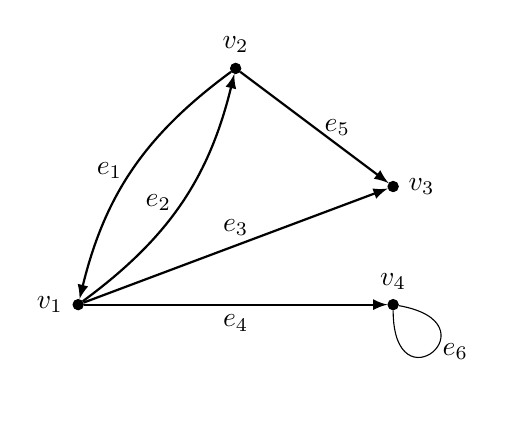
\begin{tikzpicture}[every loop/.style={}]
      \tikzset{enclosed/.style={draw, circle, inner sep=0pt, minimum size=.13cm, fill=black}}
%% Vertices
      	\node[enclosed, label={left: $v_1$}] (v1) at (0,0) {};
      	\node[enclosed, label={above: $v_2$}] (v2) at (2,3) {};
    	\node[enclosed, label={right: $v_3$}] (v3) at (4,1.5) {};
  	    \node[enclosed, label={above: $v_4$}] (v4) at (4,0) {};
%Edges
		\path[->, > = latex, thick] (v1) edge [bend right=20] node[midway, left] {$e_2$} (v2);
		\path[->, > = latex, thick] (v2) edge [bend right=20] node[midway, left] {$e_1$} (v1);
		\path[->, > = latex, thick] (v1) edge node[midway, above] {$e_3$} (v3);
		\path[->, > = latex, thick] (v1) edge node[midway, below] {$e_4$} (v4);
		\path[->, > = latex, thick] (v2) edge node[midway, right] {$e_5$} (v3);
		\path (v4) edge [out=270,in=350,looseness=35] node[right] {$e_6$} (v4);
	\end{tikzpicture}
	\caption{Orienteret graf.}
	\label{fig:orienteret}
\end{figure}


Der kan foruden disse to også være tale om \emph{blandede grafer}, som er grafer med både orienterede og ikke-orienterede kanter. Orienterede grafer kan ligesom ikke-orienterede grafer indeholde løkker og flere ensrettede kanter, der er incident med det samme par knuder, men hvis dette ikke er tilfældet, kaldes det en orienteret simpel graf. En orienteret simpel graf må også indeholde to modsatrettede kanter mellem det samme knudepar. Dermed kan en kant gå fra $v$ til $u$, selvom en anden kant går fra $u$ til $v$. Hvis der derimod optræder løkker eller flere ensrettede kanter mellem et eller flere knudepar, kaldes det en \emph{orienteret multigraf}.  
Egenskaberne for de forskellige grafer kan ses herunder:


\begin{center} \label{tab:typer}
\begin{tabular}{ |p{4cm}|p{3cm}|p{3cm}|p{2cm}|  }
 \hline
 \multicolumn{4}{|c|}{Grafer} \\
 \hline
 Type & Kanter & Flere kanter per knudepar tilladt & Løkker tilladt\\
 \hline
 Simpel graf   & Ikke-orienterede    & Nej &   Nej\\
 Multigraf &   Ikke-orienterede & Ja   & Nej\\
 Pseudograf & Ikke-orienterede & Ja &  Ja\\
 Simpel orienteret graf    & Orienterede & Nej &  Nej\\
 Orienteret multigraf &  Orienterede  & Ja & Ja\\
 Blandet graf & Ikke-orienterede og orienterede  & Ja   & Ja\\
 \hline
\end{tabular}
\end{center}

%Fordi kanterne i grafer med orienterede kanter er ordnede par, kan definitionen af knudens grader være antallet af kanter, der har denne knude som startknude, eller antallet af kanter, der har denne knude som endeknude:
%
%\begin{defn} [Graden af en orienteret graf] 
%I en graf med orienterede kanter er ind-graden, betegnet ved $\mathrm{deg}^{-}(v)$, antallet af kanter med $v$ som deres endeknude. Ud-graden, betegnet ved $\mathrm{deg}^{+}(v)$, er antallet af kanter med $v$ som deres startknude.
%\end{defn}

Vi vil i projektet beskæftige os med orienterede grafer, da det er denne type, vi bruger til optimering af gaslageret. 
